%!TEX root = ../docu.tex
\section{Projektplanung}
\label{proj}

\subsection{Arbeitspakete und Planung}
Bevor man mit der Arbeit an einem Projekt beginnen kann, stellt sich die Frage, wie Programmfeatures implementiert und Fehler beseitigt werden sollen. Außerdem müssen Aufgaben an verschiedene Personen verteilt werden.

Hierfür gibt es viele Vorgehensweisen. Eine der Häufigsten ist das Anfertigen von sogenannten Arbeitspaketen. Diese beinhalten das vorher definierte Ziel und jene Schritte, die zur Erreichung des Ziels nötig sind und welche Anforderungen das Ziel erfüllen muss.

Ein solches Arbeitspaket wird anschließend bewertet und im Aufwand eingeschätzt. Das so erstellte Arbeitspaket wird jetzt einem Bearbeiter zugeteilt.

Abhängigkeiten von Arbeitspaketen oder solche, die aufeinander aufbauen spielen eine gesonderte Rolle. Schnittstellen zwischen verschiedenen, in den Paketen implementierten Programmkomponenten müssen genau definiert werden, um spätere Fehler oder Inkompatibilität auszuschließen.

Die Verwaltung der Pakete und Zuweisung variiert je nach Größe des Teams. Weit verbreitet sind Systeme wie Trac\footnote{http://trac.edgewall.org/}, Bugzilla\footnote{http://www.bugzilla.org/} oder Redmine\footnote{http://www.redmine.org/}. Für ein Team mit kleinerer Anzahl von Mitgliedern empfehlen sich solche Systeme nicht.

Die Wartung und Konfiguration ist zu aufwendig. Die Kosten von Zeit und entstehender Nutzen stehen in keinem vertretbaren Verhältnis.

Für die Umsetzung des Projektes wurde daher das Managementtool namens Trello\footnote{https://trello.com/} eingesetzt. Es realisiert eine Managementmethode namens \textit{Kanban} welche von Automobilhersteller Toyota entwickelt wurde.

\subsubsection{Kanban}

Die Funktionsweise von Kanban wird auf ein paar wesentliche Bestandteile differenziert. Zunächst werden Stadien definiert. Je nach Projektumgebung variieren diese Stadien. Für die Entwicklung von Anwendungen sind folgende Stadien ausreichen. 

\begin{itemize}
	\item Zu Beginn ist ein Paket im Stadium \textit{nicht zugewiesen} beziehungsweise \textit{neu}.
	\item Das nächste Stadium ist \textit{zugewiesen} gefolgt vom \textit{in Bearbeitung}.
	\item Anschließend wandert das Arbeitspaket in das Stadium \textit{Test} und von dort aus in \textit{beendet}.
\end{itemize}

Das System ist übersichtlich da alle Pakete auf einen Blick einsehbar. Des Weiteren ist ersichtlich welche Person für das jeweilige Arbeitspaket zuständig ist und es bearbeitet. Durch die Position eines Paketes ist sofort erkennbar in welchen Stadium sich gerade ein Paket befindet.

Der Vorteile von Kanban liegt an der hohen Transparenz der Arbeitspakete und deren gegenwärtigen Status. Die Einführung und Umsetzung sind ressourcenschonend und schnell. Der Umgang mit Kanban ist leicht zu erlernen und gerade für kleiner Teams zu empfehlen.

\begin{figure}
\begin{center}
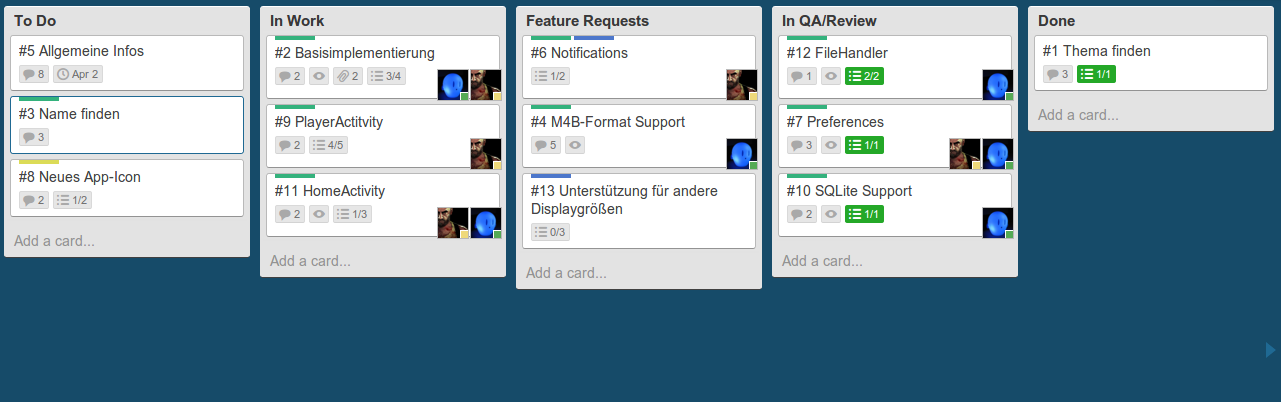
\includegraphics[scale=0.35]{images/kanban}
\caption{Kanbanboard mit verschiedneen arbeitspacketen}
\label{kanban}
\end{center}
\end{figure}

In Abbildung \ref{kanban} ist ein Kanban-Board abgebildet. Aufgaben werden dort auf Karten, die Arbeitspakete repräsentieren dokumentiert. Diese durchlaufen verschiedene Stadien und wandern von der linken zu rechten Seite des Boards.

Abgeschlossene Pakete werden nach einiger Zeit vom Brett genommen um die Übersichtlichkeit weiterhin zu gewährleisten. Solche Boards werde in Papierform oder auch auf elektronischen Wege simuliert. Weitere Einzelheiten könne aus der Literaturquelle \cite{9783898647304} entnommen werden.

\subsection{Entwicklungsumgebung}

Für das Arbeiten mit der umfangreichen Android API empfiehlt es sich eine Entwicklerwerkzeuge wie Eclipse zu verwenden. Dies gewährleistet einen schnellen Umgang mit allen Bestandteilen des Android SDK.

Des Weiteren wird die Auswertung von LOG-Daten durch das SDK schnell und Fehler somit eher identifiziert. Ähnlich wie bei der Entwicklung von Java Anwendungen ist es möglich Test zu implementieren und dadurch Fehlererkennung und dessen Beseitigung zu betreiben.

Eclipse bietet eine automatische Vervollständigung für Quellcode und eine Typprüfung vor der Kompilierung des Codes. Es ist weiterhin in der Lage viele Codeabschnitte automatisch zu erzeugen und somit Entwicklungsschritte zu erleichtern.

Wichtig bei der Arbeit mit einer IDE\footnote{Integrated Development Environment} wie Eclipse ist die Integration des SDKs um die für die Entwicklung von Android Applikationen bereitgestellten Werkzeuge nutzen zu können. Hierzu gehören verschiedene Debugger sowie Kompilierwerkzeuge, welche dem Entwickler Hilfestellung leisten.

\subsection{Versionsverwaltung des Quellcode}

Die Versionierung von Quellcode spielt eine große Rolle bei der Entwicklung von Software. Hierbei werden Änderungen am Quellcode zeitlich erfasst um einen chronologischen Verlauf von Änderungen festzuhalten und die Aktualität des Codes zu gewährleisten.

Für diesen Zweck gibt es verschiedene Lösungsmöglichkeiten. Weit verbreitet sind die Versionsverwaltungssysteme SVN\footnote{http://subversion.apache.org/} und GIT\footnote{http://git-scm.com/}.
SVN ist ein zentrales Versionsverwaltungssystem für Dateien. Es gibt einen zentralen Versionierungsserver zudem sich Klienten verbinden und Änderungen einreichen werden.

Die Wahl für die Versionsverwaltung viel auf GIT. GIT verfolgt eine andere Strategie. Änderungen werden dezentral verwaltet. Im folgenden Kapitel werden die wesentlichen Aspekte von GIT genannt.

\begin{description}

\item[Kein zentraler Server] \hfill \\
Jeder Benutzer hat eine exakte Kopie der Versionierung und ihren Verlauf. Alle Arbeiten werden daher größtenteils ohne Netzwerkzugriff ausgeführt.

\item[Datenaustausch] \hfill \\
Der Austausch von Daten wird über viele Protokolle und Arten abgewickelt. Der Austausch ist sehr flexibel und sicher, wenn für die Übertragung geeignete, abgesicherte Protokolle verwendet werden.

\item[Kryptographische Sicherheit der Projektgeschichte] \hfill \\
Während des Versionierungprozesses wird ein eindeutiger Hash erzeugt, welcher den gesamten Verlauf zur aktuellen Version wiederspiegelt eine nachträgliche Änderung ist somit nicht möglich und es ist ausgeschlossen, dass sie verschleiert wird. Gelöschte Informationen bleiben erhalten und können wiederhergestellt werden.
\end{description}

Durch die Dezentralisierung der Versionierung muss dennoch ein Austausch der Daten zwischen den Teammitgliedern gewährleistet werden. Hierfür gibt es verschiedene Möglichkeiten, unter anderem eine gemeinsame Austauschstelle. Diese Austauschstellen fungieren als Vermittel- und Sammelpunkte. Es besteht die Möglichkeit solch einen Punkt selber zu betreiben oder kostenlose Anbieter wie GitHub\footnote{https://github.com/} zu verwenden.